\chapter{相关研究综述}
\label{cha:review}

\section{深度学习技术}
\label{sec:review-deeplearning}
%深度学习技术综述
在过去的几十年,构建机器学习系统需要经验丰富的领域专家来设计特征提取器,人为设计特征表示的过程费时费力,深度学习方法则不需要人工设计特征提取器,而是由及其自动获得。深度学习是一种多层表示学习方法,用简单的非线性模块构建而成,这些模块将上一层表示转化为更高层、更抽象的表示,当一个学习系统由足够多这样简单的非线性模块构建时,可以学习复杂的功能。
%深度学习关键技术和概念
\subsection{卷积神经网络}

\subsection{监督学习算法}
\subsection{反向传播算法}
\subsection{特征提取器}

\begin{figure}[H]
\centering
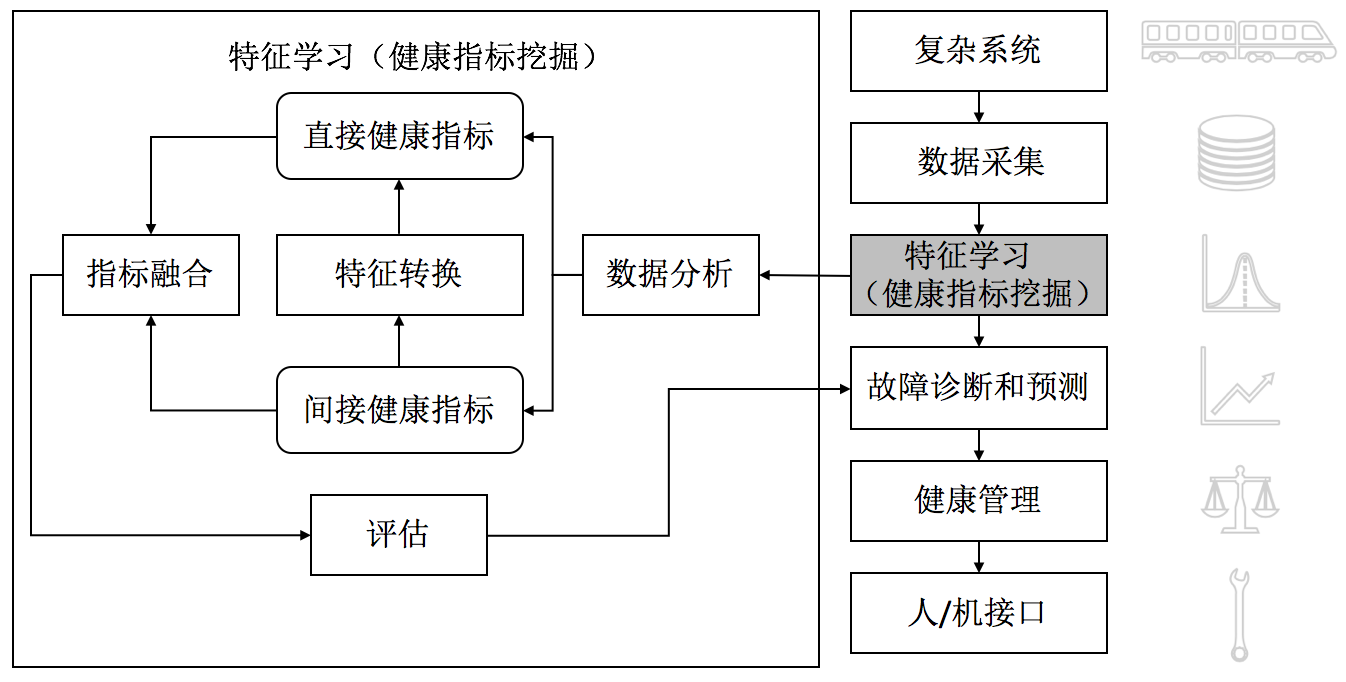
\includegraphics[scale=0.5]{figures/phm-framework.png}
\caption{PHM 系统工程}
\label{fig:phm-framework}
\end{figure}
故障预测是 PHM 的核心要义,其划分大同小异,比如Si 等人将故障预测方法分为四类,即基于实验的、数据驱动的、基于物理模型的和混合的故障预测方法\cite{si2011remaining};Lee 等人划分为三类,即基于模型的、数据驱动的和混合的故障预测方法\cite{lee2014prognostics};彭宇等人分为三类,即基于模型的、数据驱动的和基于统计可靠性的故障预测方法\cite{彭宇2010故障预测与健康管理技术综述};Pecht 等人分为两类,即基于模型的和数据驱动的故障预测方法\cite{pecht2010prognostics}。为便于讨论和研究,本文统一将故障预测方法划分为以下两类:

%\subsection{时间序列数据分析和特征学习方法}
\section{物体检测算法}
\label{sec:ts-representation-review}
% 时间序列的普遍性和重要性
% 时间序列的定义
% 时间序列分析的一般流程:数据采集 + 预处理 + 特征学习 + 任务
% 本文主要研究:预处理和特征学习,详细讨论
% 时间序列数据预处理方法:主要参考两本书
% 时间序列特征学习方法:按照现有分类进行概述

本文统一采用{\heiti 时间序列挖掘}这一术语表示对时间序列数据的开采利用过程,关键流程归纳为图\ref{fig:tsm-framework},主要包含数据采集、特征学习及应用三个环节。其中,特征学习是数据得以有效利用的关键,一直是研究热点和难点\cite{langkvist2014review}。

\begin{figure}[H]
\centering
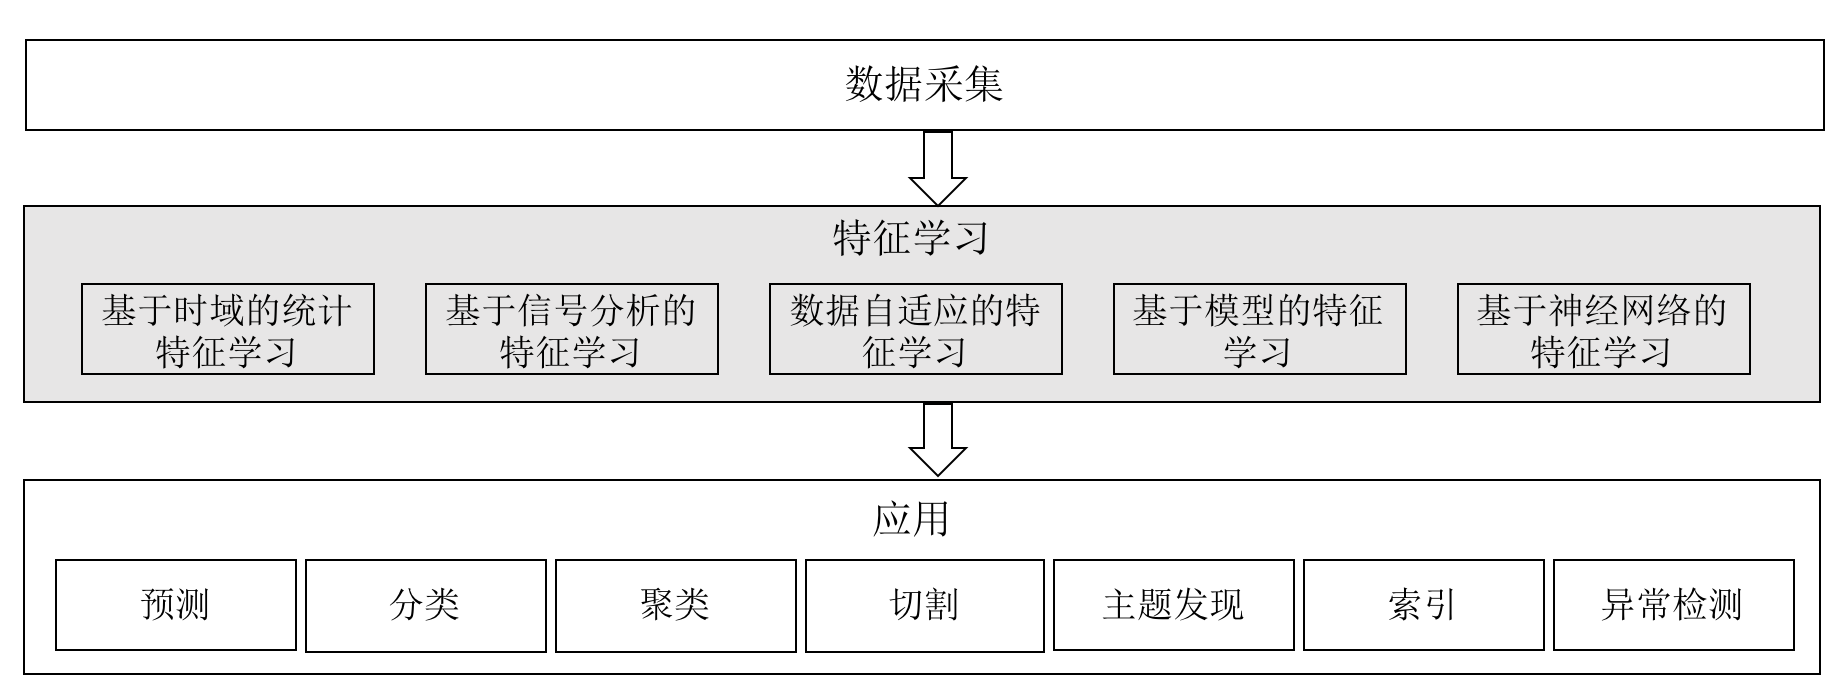
\includegraphics[scale=0.45]{figures/tsm-framework.png}
\caption{时间序列挖掘流程}
\label{fig:tsm-framework}
\end{figure}

\subsection{单阶段的物体检测算法}

单阶段物体检测

\subsection{两阶段物体检测算法} 

% 特征学习的定义
% 特征学习的普遍型和重要性
% 术语的统一
% 按分类描述方法
两阶段物体检测算法


\section{训练加速算法}
\label{sec:sr-review}

% 系统的变迁有两种。其中缓慢接近相变点的过程是可预测的。
% 尽管临界相变很难被预测,但由于全球都在关注生态系统的可持续发展,因此已有很多致力于识别临界相变早期预警特征的研究。
 Down,CSD)\cite{scheffer2009early,dakos2008slowing}和偏斜度增加\cite{guttal2008changing}这样的早期预警特征。其中CSD对早期预警特征的解释最为全面,可概括为,当系统临近临界相变点时,系统在受到外界干扰后恢复到正常状态的速度会变慢,如图\ref{fig:csd-early-warning-signal}所示,并表现出以下几个普适的早期预警特征:
\begin{itemize}
  \item 在时间序列上前后状态变得越来越相似,表现为自相关性增加。
  \item 系统在平衡点来回波动,有新状态出现的征兆,表现为歪斜率增加。
  \item 系统存在极不稳定的现象,表现为方差增大。
\end{itemize}
\begin{figure}[H]
\centering
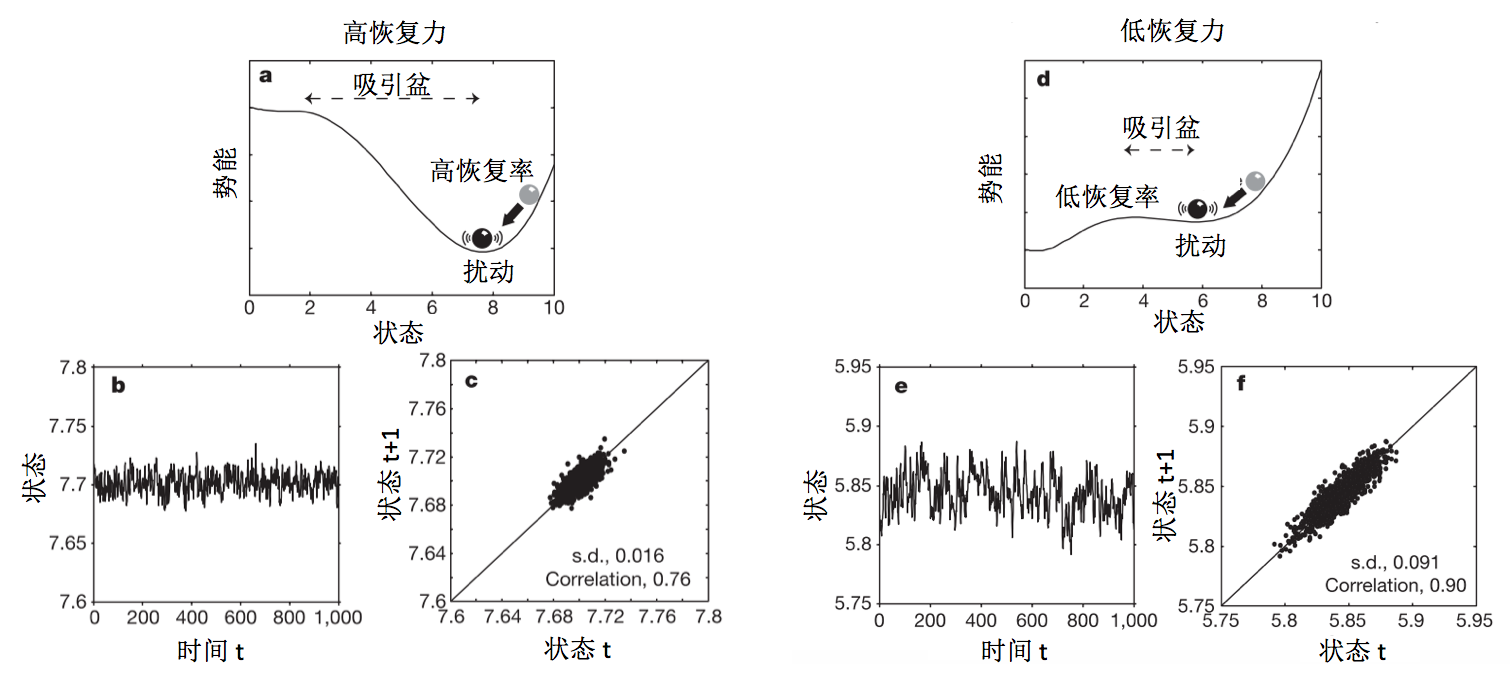
\includegraphics[scale=0.5]{figures/csd-early-warning-signal.png}
\caption{系统临近临界相变状态的特征示意图\cite{scheffer2009early}}
\label{fig:csd-early-warning-signal}
\end{figure}


\section{推理加速算法}
\label{sec:gan-review}
推理加速算法


\begin{figure}[H]
\centering
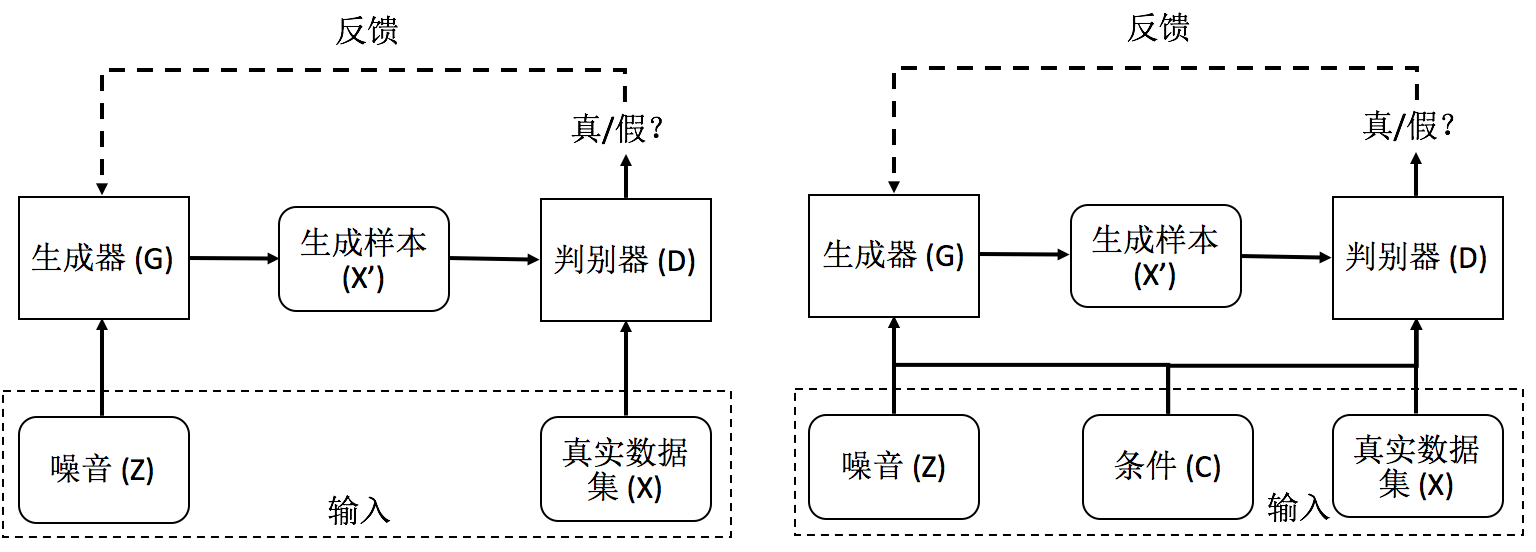
\includegraphics[scale=0.5]{gan-gan.png}
\caption{(左)生成式对抗网络,(右)条件生成式对抗网络}
\label{fig:gan-gan}
\end{figure}

\begin{equation}
\label{eq:gan-objective-function}
  \min_{G}\max_{D} V(D,G) = \mathbb{E}_{x \sim P_{data}(\bf{x})}[log(D(x))] + \mathbb{E}_{z \sim P_{z}(\bf{z})}[log(1-D(G(z)))]
\end{equation}

